\chapter{Análise de Resultados} \label{ch:analise_resultados}

Este capítulo apresenta a análise dos resultados obtidos a partir do desenvolvimento da linguagem proposta, organizados com relação aos objetivos específicos estabelecidos na \autoref{sec:objetivos}. Ele está dividido em três seções, incluindo a análise geral da implementação, as decisões de desenvolvimento e seus impactos, e por fim, a viabilidade e limitações da solução proposta, determinando se os objetivos do trabalho foram alcançados.

\section{Análise Geral da Implementação da Solução}

A implementação do protótipo de interpretador para a linguagem proposta se mostrou muito parecida com a implementação de interpretadores de linguagens tradicionais. Isso se deve ao fato dele possuir todas as fases genéricas de um interpretador tradicional implementadas, já que foi feito com base na primeira metade do livro \textit{Crafting Interpreters}, e consequentemente feito com base em Jlox \cite{craftinginterpreters}.

Saindo do escopo de fases de um interpretador e indo mais a fundo na implementação, também foi possível observar semelhanças de sintaxe com linguagens tradicionais. Um exemplo disso é a sintaxe de declaração de sistemas, que é muito parecida com a sintaxe de declaração de funções em Jlox, Rust, e muitas outras linguagens \cite{rustbook,craftinginterpreters}.

Usando regras de produção, a figura \ref{fig:decl_sistema_funcao} demonstra a semelhança entre a sintaxe de declaração de sistemas na linguagem proposta e a sintaxe de declaração de funções em Jlox. Nota-se que há apenas duas diferenças: a palavra-chave \texttt{system} no lugar de \texttt{fun} e a sintaxe de \textit{query} no lugar da lista de parâmetros.

\begin{figure}[H]
	\centering
	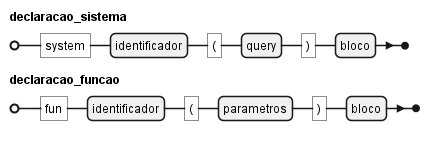
\includegraphics[width=0.45\textheight]{../diagrams/decl_sistema_funcao.png}
	\caption{Diagrama de sintaxe comparando declaração de sistemas e de funções.}
	\fonte{Elaboração própria com PlantUML feita com base no interpretador nosso e no de Jlox \cite{craftinginterpreters}.}
	\label{fig:decl_sistema_funcao}
\end{figure}

Vale ressaltar que semelhanças como essa estão presentes em outras partes da sintaxe da linguagem proposta, e foram intencionalmente feitas para facilitar a legibilidade e a facilidade de escrita através da familiaridade com outras linguagens, conforme discutido na \autoref{sec:design_linguagem}.

Fora as semelhanças, as diferenças na implementação da linguagem proposta foram encontradas principalmente na semântica e na pragmática \cite{designconceptsinlanguages}, que foram adaptadas para suportar os conceitos de ECS.

Ainda no exemplo de declaração de sistemas, a semântica foi feita de forma que o interpretador reconheça um sistema como uma função que atua sobre entidades e seus componentes de forma automática. Já a pragmática foi feita através da ligação da sua sintaxe com a API da biblioteca de ECS Flecs.

A fim de melhor documentar o processo de desenvolvimento da implementação, a seção seguinte detalha as principais decisões feitas durante o desenvolvimento do interpretador.

\section{Decisões de Desenvolvimento e seus Impactos}

Esta seção tem a finalidade de documentar as principais decisões tomadas durante o desenvolvimento do interpretador em um só lugar, possivelmente servindo de referência para trabalhos futuros. Para cada decisão, será descrito o objetivo da decisão, a decisão em si, seu impacto no protótipo, e, caso aplicável, alternativas relevantes.

\subsection{Escolha da Linguagem de Implementação}

\begin{itemize}
	\item \textbf{Objetivo}: Escolher uma linguagem de programação adequada para implementar o interpretador, considerando fatores como suporte de bibliotecas, estruturas de dados expressivas e familiaridade do desenvolvedor;
	\item \textbf{Decisão}: A linguagem escolhida foi Rust, devido ao seu suporte a \textit{Algebraic Data Types} através de \texttt{enums} \cite{rustbook}, seu ecosistema com as bibliotecas necessárias, e a familiaridade do desenvolvedor com a linguagem;
	\item \textbf{Impacto}: A escolha de Rust tornou o processo de depuração extremamente previsível devido ao seu sistema de tipos rígido, além de permitir abstrações mais expressivas através de \texttt{enums} \cite{rustbook}.
\end{itemize}

\subsection{Escolhas de \textit{Design} da Linguagem}

\begin{itemize}
	\item \textbf{Objetivo}: Integrar o ECS no \textit{design} da linguagem da forma mais simples e intuitiva possível, visto que o foco do trabalho está na implementação do interpretador;
	\item \textbf{Decisão}: O \textit{design} da linguagem foi feito adaptando a sintaxe de linguagens imperativas tradicionais para suportar os conceitos base de ECS: entidades, componentes e sistemas. Adicionalmente, a semântica e pragmática também seguem os conceitos de ECS.
	\item \textbf{Impacto}: Toda a sintaxe proposta pelo \textit{design} foi implementada e conseguiu servir de base para a semântica e pragmática necessárias para a integração com a biblioteca de ECS.
	% Como analisado na \autoref{tab:caracteristicas_nosso_design}, que compara \textit{design} da linguagem proposta com a biblioteca Flecs, nota-se que nosso \textit{design} marca todas as características relacionadas ao critério de legibilidade, porém não marca nenhuma característica relacionada aos critérios de facilidade de escrita e de confiabilidade.
\end{itemize}

\subsection{Representação das Abstrações Internas}

\begin{itemize}
	\item \textbf{Objetivo}: Definir as estruturas de dados internas para representar as abstrações da linguagem proposta, como \textit{tokens}, expressões e instruções.
	\item \textbf{Decisão}: Utilizar \texttt{enums} do Rust para representar as abstrações internas, aproveitando o suporte a \textit{Algebraic Data Types} da linguagem \cite{rustbook}.
	\item \textbf{Alternativa}: Utilizar \texttt{structs} com campos para representar o tipo de cada abstração, como é feito em Jlox \cite{craftinginterpreters}. Essa alternativa foi descartada devido à superioridade dos \texttt{enums} quanto a código mais robusto.
	\item \textbf{Impacto}: A escolha de \texttt{enums} tornou o código mais robusto, já que em conjunto com \texttt{match}, o compilador do Rust consegue garantir que todos os casos possíveis de cada abstração sejam tratados \cite{rustbook}.
\end{itemize}

\subsection{Estratégia de Análise Léxica}

\begin{itemize}
	\item \textbf{Objetivo}: Definir a estratégia de análise léxica para converter o código-fonte em uma sequência de \textit{tokens}. Idealmente, ela deve ser simples de implementar, já que o trabalho se trata de um protótipo.
	\item \textbf{Decisão}: A estratégia escolhida foi a implementação de um \textit{lexer} manual com \textit{iterators}, inspirado na implementação do Jlox \cite{craftinginterpreters}.
	\item \textbf{Alternativa}: Utilizar uma biblioteca geradora de \textit{lexers}. Inicialmente, a implementação do \textit{lexer} foi feita com a biblioteca Logos, porém, na época em que foi utilizada, não havia documentação suficiente sobre integração de erros customizados com a biblioteca, o que levou a decisão de implementar um \textit{lexer} manualmente.
	\item \textbf{Impacto}: A implementação do \textit{lexer} manual foi relativamente simples, com em torno de 180 linhas de código, e permitiu a implementação de erros customizados. Porém, caso a biblioteca Logos tivesse documentação suficiente na época, a implementação poderia ter sido mais simples e com menos linhas de código, como é possivel inferir dos exemplos na documentação da biblioteca \cite{logos}.
\end{itemize}

\subsection{Estratégia de Análise Sintática}

\begin{itemize}
	\item \textbf{Objetivo}: Definir a estratégia de análise sintática para converter a sequência de \textit{tokens} em uma AST. Idealmente, ela deve ser simples de implementar, já que o trabalho se trata de um protótipo.
	\item \textbf{Decisão}: Diferente do \textit{lexer}, a implementação do \textit{parser} foi feita com uma biblioteca, Chumsky, que expõe uma API para criar \textit{parsers} de forma declarativa \cite{chumsky}.
	\item \textbf{Impacto}: A implementação do \textit{parser} com Chumsky foi relativamente simples, principalmente quando comparada com a implementação de \textit{parsers} manuais, como o do Jlox \cite{craftinginterpreters}. Devido a natureza declarativa da biblioteca, o código do \textit{parser} ficou extremamente parecido com as regras de produção da gramática, como comentado na \autoref{sec:analise_sintatica}. Isso facilitou a implementação e a depuração do \textit{parser}, que ficou com em torno de 120 linhas de código.
\end{itemize}

% TODO!
% \subsection{Estratégia de Interpretação}

% \begin{itemize}
% 	\item \textbf{Objetivo}:
% 	\item \textbf{Decisão}:
% 	\item \textbf{Impacto}:
% \end{itemize}

\subsection{Escolha da Biblioteca de ECS}

\begin{itemize}
	\item \textbf{Objetivo}: Escolher uma biblioteca de ECS adequada para integrar com o interpretador, considerando fatores como suporte da linguagem de implementação e documentação extensa;
	\item \textbf{Decisão}: A biblioteca escolhida foi Flecs, devido ao seu suporte a Rust através de \textit{bindings} e sua documentação extensa \cite{flecs}. Adicionalmente, o autor dessa biblioteca é o mesmo dos vários artigos sobre ECS usados neste trabalho. Além disso, Flecs é uma das poucas bibliotecas de ECS que suporta relacionamento entre entidades, o que será útil para as sugestões de trabalhos futuros \cite{flecs}.
	\item \textbf{Impacto}: A escolha da biblioteca Flecs facilitou sua integração com o interpretador, devido a sua documentação e artigos relacionados do autor. Porém, pelo fato de seu \textit{binding} para Rust não possuir declaração de componentes de forma dinâmica, a integração exigiu uma estratégia incomum, como descrita na \autoref{sec:interpretacao} \cite{flecs}.
\end{itemize}

% TODO!
% \subsection{Representação Interna de Entidades, Componentes e Sistemas}

% \begin{itemize}
% 	\item \textbf{Objetivo}:
% 	\item \textbf{Decisão}:
% 	\item \textbf{Impacto}:
% \end{itemize}

\section{Viabilidade e Limitações da Solução}

% TODO! Escrever esta seção por conta própria. O abaixo é só um rascunho do Gepeto.

% Por fim, esta seção avalia a viabilidade e limitações da solução proposta, determinando se os objetivos do trabalho foram alcançados.

% A implementação do protótipo de interpretador para a linguagem proposta conseguiu atingir todos os objetivos específicos estabelecidos na \autoref{sec:objetivos}. A seguir, cada objetivo específico é revisitado e avaliado:

% \begin{itemize}
% 	\item \textbf{Objetivo 1}: Pesquisar e analisar conceitos de ECS e linguagens de programação para embasar o desenvolvimento da linguagem proposta.
% 	\begin{itemize}
% 		\item \textbf{Avaliação}: Este objetivo foi alcançado através da pesquisa e análise dos conceitos de ECS, linguagens de programação, e interpretadores, conforme documentado na \autoref{ch:fundamentacao_teorica}.
% 	\end{itemize}
% 	\item \textbf{Objetivo 2}: Propor um \textit{design} de linguagem que integre os conceitos de ECS de forma simples e intuitiva.
% 	\begin{itemize}
% 		\item \textbf{Avaliação}: Este objetivo foi alcançado através do desenvolvimento do \textit{design} da linguagem, conforme documentado na \autoref{ch:design_linguagem}.
% 	\end{itemize}
% 	\item \textbf{Objetivo 3}: Implementar um protótipo de interpretador para a linguagem proposta, utilizando uma biblioteca de ECS.
% 	\begin{itemize}
% 		\item \textbf{Avaliação}: Este objetivo foi alcançado através da implementação do protótipo de interpretador, conforme documentado na \autoref{ch:implementacao}.
% 	\end{itemize}
% \end{itemize}

% Com base na análise acima, conclui-se que a solução proposta é viável e que os objetivos do trabalho foram plenamente alcançados. O protótipo de interpretador desenvolvido demonstra a integração bem-sucedida dos conceitos de ECS na linguagem proposta, atendendo aos requisitos estabelecidos no início do trabalho.
